\section{Ping Pong Ball Bombe}

\margininbox{Smer0}{
     \begin{itemize}
    \item Aljošha Bončina
    \item Erik Bončina
    \item Emil Frankič
    \item Jarvist Frost
    \item Izi Možir
    \item Zdenko Rejec
    \item Richard Venn
    \item Silan    
    \end{itemize}}{\explo}


A Slovene super-action was in the making, the Shepherd's huts stocked
with drink and the young JSPDT bouncing down to -200 m in
\passage{Primadona} to improve the rigging. The plan was to (mainly)
investigate leads off \passage{Smer0}/\passage{Smer1} in \passage{Primadona} where on a JSPDT
trip in Autumn 2006 (joined by Tetley \& Jarv from IC) a large rift with
an approx 40 m pitch was found - most tellingly, with water visible at
the bottom. Finding a constant stream this shallow in \passage{Mig} was unheard
of. Meanwhile, a smaller team would head to \passage{Bikini Carwash} at the
end of \passage{Exhibition Road} in the main system and aid climb to see if the
passage continued.

The more curious aspect of this mission was the Ping Pong Ball Bombe, a
plan to take ping pong balls down \passage{Primadona} \& set fire to
them. The noxious smell hopefully providing a connection. Alas, the
\passage{Sistem Migovec} team that was to detect with their noses, also contained the most
hardened smokers who spent their time sniffing the air in between
dragging on filterless roll ups!

With mammoth organisation, Rik and Jarv were dispatched down via text
message from the \passage{Bivi} to \passage{Kal}, meeting the Slovs and stealing some bread
before crabbing across sideways to \passage{Primadona}. The boulder slope
climb was awful as ever, but I took the opportunity to build a cairn on
the edge of the cliff so that we could recognise this point from the
plateau - to help unravel the mystery of the caves below \passage{B9} spotted by
Jana \& I from the plateau the Autumn before.

So we went down in a mammoth party: Rik, Jarv, Erik, Aliosha, Izzy,
Silan, Zdenko \& Emil.

Zdenko led off with the young JSPDT. Emil was a new character to us --
with a bald head framed by round lensed glasses and a fine handlebar
moustache that dovetailed with his military demeanour, were it not for
the Slovene language I could have easily assumed him to be an old-school
English army Colonel. Bringing up the rear with Emil, we were slowed by
his enormous tackle sac, stuffed full of bread and cheese I could only
assume. About 150 m in, standing on a traverse line above a pitch, I was
handed a full mineral water bottle from the depths of this magic sack.
``What is it?'' I asked. ``Mmm\ldots{} made with fruits\ldots{} and a
kilo of Med (honey)\ldots{} it's dobra!'' Ah, I thought, some marvellous
mountain tea fortified with a shed load of honey - just perfect to give
an energy boost and fight off the dehydration. \bignote{I chugged it back. Tea it
was not. Double distilled Zjganja with a kilo of honey dissolved in it
it was}.

Once at the pushing front we found we were rather limited with gear --
just one bolt kit. Rik set to work with Izzy to get down the pitch.
Zdenko and the Eric/Aliosha brotherhood set off for the end of \passage{Smer0}
(passed where \passage{Smer1} reconnected to it) to look at the climb that
currently ended the passage. Jana, Emil \& myself traversed over the
pitch (which was a truly frightening undertaking - walls over a metre
apart with a 40 m drop down) and went to look at where the water which
trickled down the opposite side came from. From the pools of water we
found a 2 m climb into an old dry silted phreatic system leading left
facing towards the end of \passage{Smer0}, starting just before where \passage{Smer1}
dropped down. This branched to a small chamber with avens, a too tight
rift (from which, insanely enough, emanated sounds of Rik bolting) and a
chamber with a larger, aid climbable, aven. Alas, with no spare rigging
gear for the climb, and no survey instruments, there wasn't much more
for us to do but go back to Rik.

Rik \& co had made it down about 20 m to a ledge where he put in a
rebelay bolt. He reckoned he could see the floor a further 20 m from
there. He was rather put off by the avalanche of rocks that came down
when people went over the crazy free traverse. The team that went to the
end of \passage{Smer0} was already back, and getting cold waiting around with
nothing to do we set off out in small groups. Rik finished the rebelay
bolt and headed back up, as the guys he was with were getting cold.

In the end we didn't burn the Ping Pong Bombes, as \passage{Primadona}
appeared to be breathing `out' in all the bits a draught was detectable.

As well as the spirits, Emil had another mineral water bottle filled
with white wine, for the journey out. When he returned to the mountain
hut well gone midnight he did not look particularly well. \bignote{One can only
assume he burnt through his hangover on the pitches out}!

\passage{Primadona} is I'm sure an absolutely amazing cave system, whose
secrets have only been very partially unlocked. Unfortunately I fear it
will require a heroic effort to make easier access (possibly by
reactivating the abseil route, or finding a better abseil way down via
\passage{B9}/\passage{Planika}/\passage{Monatip}) to allow the dozens of small trips necessary to
properly relearn the cave system, recapturing the knowledge lost with
the retirement from caving of the `middle-aged' JSPDT who mainly
explored \passage{Primadona}.

\name{Jarvist Frost}


\begin{pagefigure}
      \checkoddpage \ifoddpage \forcerectofloat \else \forceversofloat \fi
      \centering
              \frame{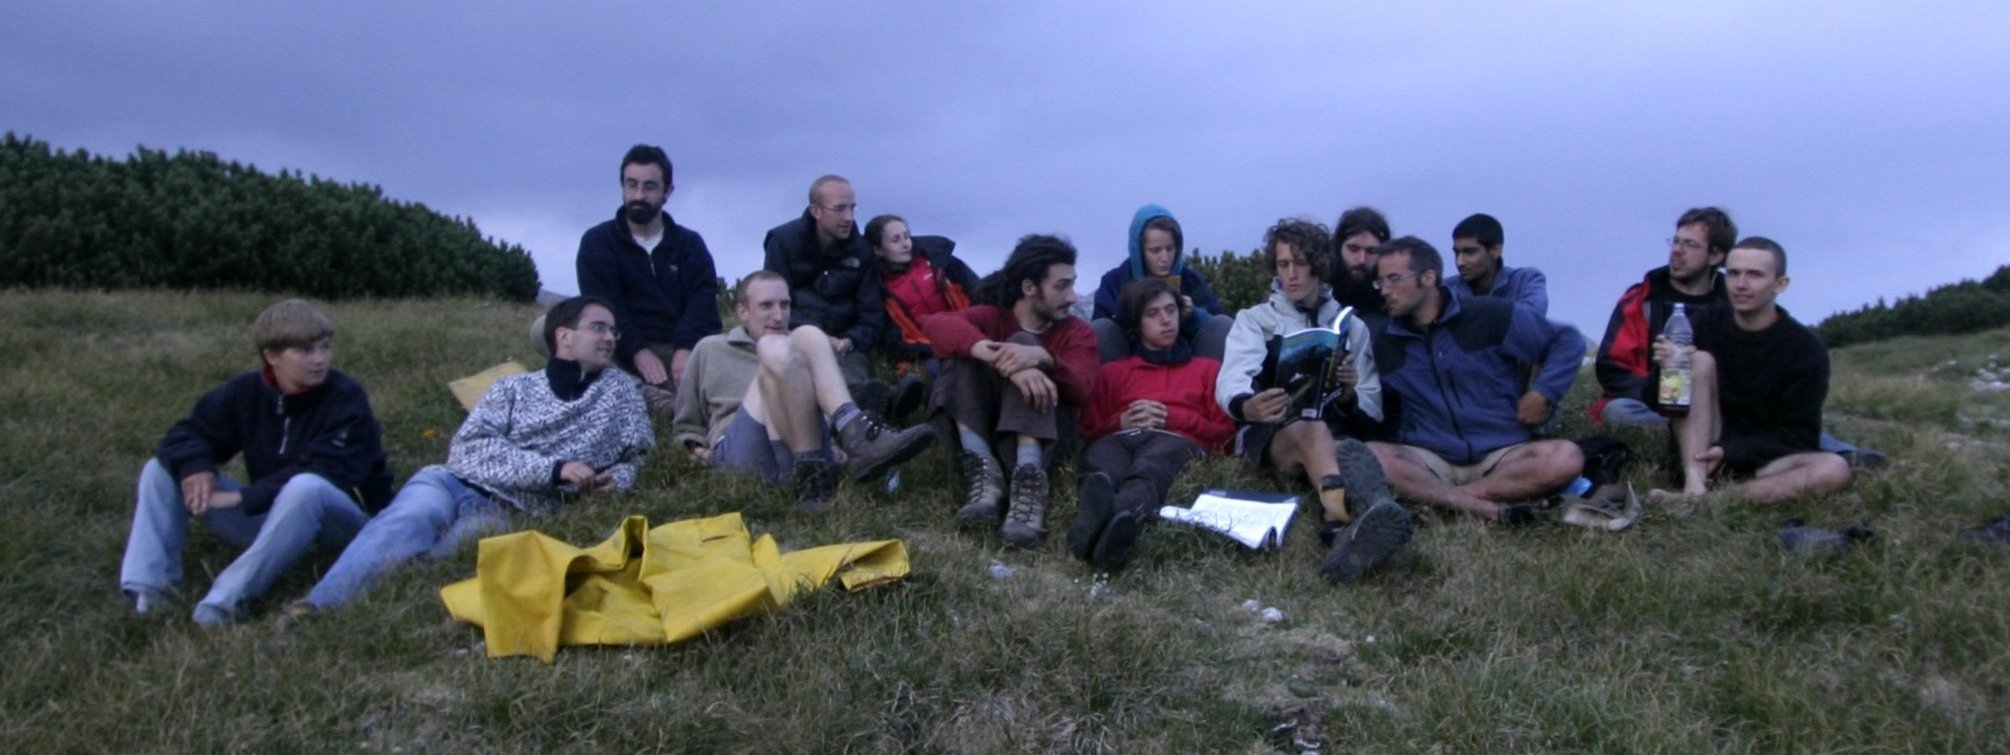
\includegraphics[width=\linewidth]{2007/ping_pong_ball_bombe/martin mcgowan -sunset shot--crop.jpg}} 
  \caption{Jarv gives a 'Sermon on the Mount', \passage{Migovec} style, by reading from \textit{The Hollow Mountain} (published 2007) to the masses. \pic{Martin McGowan}}
\end{pagefigure}

